\section{Population Synthesis}\label{app:pop_synth}

In this section we summarise the main assumptions and settings that we use when performing population synthesis for this work. For a more general overview of every setting see \citet{Broekgaarden+2021}.

\subsection{Initial conditions}

We simulate between 1 and 100 million massive binaries for 50 metallicities equally spaced in log space between $Z \in [0.0001, 0.022]$, where $Z$ is the mass fraction of heavy elements. We simulate more binaries for higher metallicities to account for the lower formation rate of DCOs. These metallicities span the allowed metallicity range for the original fitting formulae on which COMPAS is based \citep{Hurley+2000}. This is repeated for \nMinusOneModels{} physics variations (see Section \ref{sec:variation_assumptions}) and so in total over two billion binaries were simulated.

Each binary is sampled from initial distributions for the primary and secondary masses as well as the separation. The primary mass, that is the mass of the initially more massive star, is restricted to $m_1 \in [5, 150] \unit{M_{\odot}}$, which spans the range of interest for NS and BH formation in binary systems, and drawn from the \citet{Kroupa+2001} initial mass function (IMF), $p(m_1) \propto m_1^{-2.3}$. The secondary mass, $m_2$, is drawn using the initial mass ratio of the binary, $q \equiv m_2 / m_1$, which we assume to be uniform on $[0, 1]$, therefore $p(q) = 1$ \citep[consistent e.g.\ with][]{Sana+2012}. We additionally restrict the secondary masses $m_2 \ge 0.1 \unit{M_{\odot}}$, which is approximately the minimum mass for a main sequence star. We assume that the initial separation follows a flat in the log distribution with $p(a_i) \propto 1 / a_i$ and $a_i \in [0.01, 1000] \unit{AU}$ \citep{Opik+1924, Abt+1983}. We assume that all binary orbits are circular at birth to reduce the dimensions of initial parameters. Since we focus on post-interaction binaries which will have circularised after mass transfer this is a reasonable assumption and is likely not critical for predicting detection rates \citep{Hurley+2002, deMink+2015}.

We apply the adaptive importance sampling algorithm STROOPWAFEL \citep{Broekgaarden+2019} to improve the yield of our sample. This algorithm increases the prevalence of target DCOs (BHBHs, BHNSs and NSNSs in this case) in the sample and assigns each a weight, $w$, which represents the probability of drawing it without STROOPWAFEL in effect.

\subsection{Physical assumptions in our fiducial model}\label{sec:fiducial_physics}

\textit{Stellar Evolution:} To follow the evolution of massive stars, COMPAS relies on fitting formulae by \citet{Hurley+2000} to detailed single star models by \citet{Pols+1998}. COMPAS models the evolution of stars that lose or gain mass closely following the algorithms originally described in \citet{Tout+1996} and \citet{Hurley+2002}.

\textit{Wind mass loss:} We follow the wind prescription from \citet{Belczynski+2008}, which was based on results from Monte Carlo radiative transfer simulation of \citet{Vink+2000, Vink+2001}. We use the wind mass loss rates from \citet{Vink+2001} for stars above $12500 \unit{K}$ and the rates from \citet{Hurley+2000} for cooler stars. Additionally, we use a separate, higher wind mass loss rate for luminous blue variable (LBV) stars, following \citet{Belczynski+2008}, to mimic observer LBV eruptions for stars with luminosities and  effective temperatures above the Humphrey Davidson limit. We use the Wolf-Rayet-like mass loss rate from \citet{Hamann+1998} with an additional metallicity scaling from \citet{Vink+2005} for helium stars and set $f_{\rm WR} = 1$. See Team COMPAS: J. Riley et al. (in prep), Section 3 for the explicit equations.

\textit{Mass Transfer:} In determining the stability of mass transfer we use the $\zeta$-prescription, which compares the radial response of the star with the response of the Roche lobe radius to the mass transfer \citep[e.g.][]{Hjellming+1987}. The mass transfer efficiency, $\beta \equiv \Delta M_{\rm acc} / \Delta M_{\rm don}$, is defined as the fraction of the mass transferred by the donor that is actually accreted by the accretor. We limit the maximum accretion rate for stars to $\Delta M_{\rm acc} / \Delta t \le 10 M_{\rm acc} / \tau_{\rm KH}$, where $\tau_{\rm KH}$ is the Kelvin-Helmholtz timescale of the star \citep{Paczynski+1972, Hurley+2002}. The maximum accretion rate for compact objects is limited to the Eddington accretion rate. If more mass than these rates is accreted then we assume that the excess is lost through isotropic re-emission in the vicinity of the accreting star \citep[e.g.][]{Massevitch+1975, Soberman+1997}. We assume that all mass transfer from a stripped post-helium-burning-star (case BB) onto a neutron star or black hole is unstable \citep{Tauris+2015}.

\textit{Common Envelope:} A common envelope phase follows dynamically unstable mass transfer and we parameterise this using the $\alpha$-$\lambda$ prescription from \citet{Webbink+1984} and \citet{deKool+1990}. We assume $\alpha = 1$, such that all of the gravitational binding energy is available for the ejection of the envelope. For $\lambda$ we use the fitting formulae from \citet{Xu+2010, Xu+2010a}. We assume that any Hertzsprung gap donor stars that initiate a common envelope phase will not survive this phase due to a lack of a steep density gradient between the core and envelope \citep{Taam+2000, Ivanova+2004, Klencki+2021}. This follows the `pessimistic' common envelope scenario \citep[c.f.][]{Belczynski+2007}. We remove any binaries where the secondary immediately fills its Roche lobe upon the conclusion of the common envelope phase as we treat these as failed common envelope ejections, likely leading to a stellar merger.

\textit{Supernovae:} We draw the remnant masses and natal kick magnitudes from different distributions depending on the type of supernova that occurs. For stars undergoing a general core-collapse supernova, we use the \textit{delayed} supernova remnant mass prescription from \citet{Fryer+2012}. The \textit{delayed} prescription does not reproduce the neutron star black hole mass gap and we use this as our default as it has been shown to provide a better fit for observed populations of DCOs \citep[e.g.][]{Vigna-Gomez+2018}. We draw the natal kick magnitudes from a Maxwellian velocity distribution with a one-dimensional root-mean-square velocity dispersion of $\sigma_{\rm rms}^{\rm 1D} = 265 \unit{km}{s^{-1}}$ \citep{Lyne+1994, Hobbs+2005}. We assume that stars with helium core masses between $1.6$--$2.25 \unit{M_{\odot}}$ \citep{Hurley+2002} experience electron-capture supernovae (ECSN) \citep{Nomoto+1984, Nomoto+1987, Ivanova+2008}. We set all remnant masses to $1.26 \unit{M_{\odot}}$ in this case as an approximation of the solution to Equation 8 of \citet{Timmes+1996}. For these supernovae, we set $\sigma_{\rm rms}^{\rm 1D} = 30 \unit{km}{s^{-1}}$ \citep[e.g.][]{Pfahl+2002, Podsiadlowski+2004}. We assume that stars that undergo case BB mass transfer \citep{Dewi+2002} experience extreme stripping which leads to an ultra-stripped supernova \citep{Tauris+2013, Tauris+2015}. For these supernovae we calculate the remnant mass using the \citet{Fryer+2012} prescription and use $\sigma_{\rm rms}^{\rm 1D} = 30 \unit{km}{s^{-1}}$ (as with ECSN). Stars with final helium core masses between $35$-$135 \unit{M_{\odot}}$ are presumed to undergo a pair-instability, or pulsational pair-instability supernova \citep[e.g.][]{Woosley+2007, Farmer+2019}. We follow the prescription from \citet{Marchant+2019} as implemented in \citep{Stevenson+2019} for these supernovae. We assume that kicks are isotropic in the frame of the collapsing star. We adopt a maximum neutron star mass of $2.5 \unit{M_{\odot}}$ \citep[e.g.][]{Kalogera+1996, Fryer+2015, Margalit+2017} for the fiducial model and change the \citet{Fryer+2012} prescription accordingly.

\subsection{Model variations} \label{sec:variation_assumptions}
In addition to our fiducial model for the formation of DCOs, we explore \nMinusOneModels{} other models in which we change various aspects of the mass transfer, common envelope, supernova and wind mass loss physics assumptions in order to assess the effect of their uncertainties on the overall double compact object detection rates and distributions. Each of the models varies a single physics assumption (fiducial assumptions are outlined in Section~\ref{sec:fiducial_physics}) and these models are outlined in Table~\ref{tab:physics_variations}.

Our fiducial model is labelled model \modFid{}. Models \modRangeMT{} focus on changes to the mass transfer physics assumptions. We explore the effect of fixing the mass transfer efficiency $\beta$ to a constant value, rather than allowing it to vary based on the maximum accretion rate. In models \modBetaLow{}, \modBetaMed{}, \modBetaHigh{}, in which we set the value of $\beta$ to $0.25$, $0.5$ and $0.75$ respectively. In model \modCaseBB{} we investigate the consequence of assuming that case BB mass transfer onto a neutron star or black hole is always stable rather than always unstable.

Models \modRangeCE{} focus on altering the common envelope physics. We change the common envelope efficiency parameter to $\alpha_{\rm CE} = 0.1, 0.5, 2.0, 10.0$ in models \modAlphaLowest{}, \modAlphaLow{}, \modAlphaHigh{} and \modAlphaHighest{} respectively. In model \modOpt{}, we relax our restriction that Hertzsprung gap donor stars cannot survive common envelope events, thereby following the `optimistic' common envelope scenario. We combine this with model \modCaseBB{} in model \modCaseBBOpt{}.

In models \modRangeSN{} we consider changes related to our assumptions about supernova physics. Model \modRapid{} uses the alternate \textit{rapid} remnant mass prescription from \citet{Fryer+2012} instead of the \textit{delayed} prescription. We change the maximum neutron star mass in models \modNSLow{} and \modNSHigh{} to $2$ and $3 \unit{M_{\odot}}$ respectively to account for the range of predicted maximum neutron star masses. Model \modNoPISN{} removes the implementation of pair-instability and pulsational pair-instability supernovae. In models \modSigLow{} and \modSigLower{} we decrease the root-mean-square velocity dispersion for core-collapse supernovae to explore the effect of lower kicks. Model \modNoBH{} removes the natal kick for all black holes.

Finally, in models \modRangeML{} we investigate the effect of changing our assumption about wind mass loss rates, specifically for Wolf-Rayet winds. We vary $f_{\rm WR}$ to $0.1$ and $5.0$ in models \modWRLow{} and \modWRHigh{} respectively. These values approximately span the current range of possible Wolf-Rayet wind efficiencies suggested from observations (e.g. \citet{Vink+2017}, \citet{Hamann+2019}, \citet{Shenar+2019}, \citet{Miller-Jones+2021} and van Son et al. (in prep)).

\begin{table}[htb]
    \centering
    \begin{tabular}{cl}
        \hline \hline
        Model & Physics Variation \\
        \hline \hline
        \modFid & Fiducial (see Section~\ref{sec:fiducial_physics}) \\
        \hline
        \modBetaLow & Fixed mass transfer efficiency of $\beta=0.25$ \\ 
        \modBetaMed & Fixed mass transfer efficiency of $\beta=0.5$  \\ 
        \modBetaHigh & Fixed mass transfer efficiency of $\beta=0.75$ \\ 
        \modCaseBB & Case BB mass transfer is always unstable \\
        \modCaseBBOpt & Model \modCaseBB{} + Model \modOpt{} \\
        \hline
        \modAlphaLowest & CE efficiency parameter $\alpha = 0.1$ \\
        \modAlphaLow & CE efficiency parameter $\alpha = 0.5$ \\
        \modAlphaHigh & CE efficiency parameter $\alpha = 2$   \\
        \modAlphaHighest & CE efficiency parameter $\alpha = 10$   \\
        \modOpt & HG donor stars initiating a CE survive CE \\
        \hline
        \modRapid & Fryer rapid SN remnant mass prescription \\
        \modNSLow & Maximum NS mass is fixed to $2\unit{M_{\rm odot}}$ \\
        \modNSHigh & Maximum NS mass is fixed to $3\unit{M_{\rm odot}}$ \\
        \modNoPISN & PISN and pulsational-PISN not implemented \\
        \modSigLow & $\sigma_{\rm{rms}}^{\rm{1D}}=100 \unit{km}{s^{-1}}$ for core-collapse supernova \\  
        \modSigLower & $\sigma_{\rm{rms}}^{\rm{1D}}=30  \unit{km}{s^{-1}}$ for core-collapse supernova \\ 
        \modNoBH & Black holes receive no natal kick \\
        \hline
        \modWRLow & Wolf-Rayet wind factor $f_{\rm WR} = 0.1$ \\
        \modWRHigh & Wolf-Rayet wind factor $f_{\rm WR} = 5.0$ \\
        \hline \hline
    \end{tabular}%
    \caption{A description of the \nModels{} binary population synthesis models used in this study. \modFid{} is the fiducial model, \modRangeMT{} change mass transfer physics, \modRangeCE{} change common envelope physics , \modRangeSN{} change supernova physics and \modRangeML{} change wind mass loss \citep[c.f.][Table 2]{Broekgaarden+2021}.}
    \label{tab:physics_variations}
\end{table}


\section{Detection Rate Normalisation}\label{app:rate_normalisation}
In this section we explain the normalisation process that we refer to in Section~\ref{sec:gw_detection}. From each simulated instance of the Milky Way we extract the fraction of targets that are detectable, where we define a target as one of BHBH, BHNS or NSNS that merges in a Hubble time. To convert the detectable fraction to a detection rate for the Milky Way, we write that the \textit{number} of detectable targets in the Milky Way is
\begin{equation}\label{eq:norm_frame}
    N_{\rm detect} = f_{\rm detect} \cdot N_{\rm target, MW},
\end{equation}
where $f_{\rm detect}$ is the fraction of targets in the instance that were detectable and $N_{\rm target, MW}$ is the total number of targets that have been formed in the Milky Way's history. We can further break this total down into
\begin{equation}
    N_{\rm target, MW} = \avg{ \mathcal{R}_{\rm target} } \cdot M_{\rm SF, MW},
\end{equation}
where $\avg{ \mathcal{R}_{\rm target} }$ is the average number of targets formed per star forming mass and $M_{\rm SF, MW}$ is the star forming mass of the Milky Way, meaning the total mass of every star ever formed in the Milky Way.

\subsection{Average target formation rate}
Double compact object formation is metallicity dependent, so we find the average rate as the integral over metallicity, which is given by
\begin{equation}\label{eq:norm_avg_target_formation}
    \avg{ \mathcal{R}_{\rm target} } = \int_{Z_{\rm min}}^{Z_{\rm max}} p_{Z} \mathcal{R}_{\rm target, Z} \dd{Z},
\end{equation}
where $Z_{\rm min}, Z_{\rm max}$ are the minimum and maximum sampled metallicities, $p_Z$ is the probability of forming a star at the metallicity $Z$ (which can be found using the distribution in \citealp{Frankel+2018}) and $\mathcal{R}_{\rm target, Z}$ is the number of targets formed per star forming mass,
\begin{equation}
    \mathcal{R}_{\rm target, Z} =  \frac{N_{\rm target, Z}}{ M_{\rm SF, Z} }.
\end{equation}
In practice, this integral is instead approximated as a sum over the metallicity bins that we use in our simulation. The number of targets in our sample at a metallicity $Z$, $N_{\rm target, Z}$, can be written simply as the sum of the targets' weights:
\begin{equation}
    N_{\rm target, Z} = \sum_{i=1}^{N_{\rm binaries, Z}} w_i \theta_{\rm target, i},
\end{equation}
where $w_i$ is the adaptive importance sampling weight assigned to the binary by STROOPWAFEL, $N_{\rm binaries, Z}$ is the number of binaries at metallicity $Z$ in our sample and $\theta_{\rm target, i}$ is a step function that is only $1$ when the binary is a target and otherwise $0$.

The total star forming mass at a metallicity $Z$, $M_{\rm SF, Z}$, can be written as
\begin{equation}
    M_{\rm SF, Z} = \frac{\avg{m}_{\rm COMPAS, Z}}{f_{\rm trunc}} \sum_{i=1}^{N_{\rm binaries, Z}} w_i,
\end{equation}
where $\avg{m}_{\rm COMPAS}$ is the average star forming mass of a binary in our sample and $f_{\rm trunc}$ is the fraction of the total stellar mass from which COMPAS samples, given its truncated mass and separation ranges (see Section \ref{sec:COMPAS_explained}). These truncations mean that only $f_{\rm trunc} \approx 0.2$ of the stellar mass in the galaxy is sampled from.

\subsection{Total star forming mass in the Milky Way}
It is important to distinguish between the \textit{total} mass of every star formed over the entire history of the Milky Way and the \textit{current} stellar mass in the Milky Way. Many stars born in the Milky Way are no longer living and have lost much of their mass to stellar winds and supernovae, thus the current stellar mass in the Milky Way is an underestimate of the total star forming mass.

\citet{Licquia+2015} find that the total stellar mass today in the Milky Way is $6.08 \pm 1.14 \times 10^{10} \unit{M_{\odot}}$. This total includes all stars and stellar remnants (white dwarfs, neutrons stars and black holes) but \textit{excludes} brown dwarfs. We can write that the total mass of every star every formed in the Milky Way is
\begin{equation}\label{eq:m_SF_MW}
    M_{\rm SF, MW} = (6.08 \pm 1.14) \times 10^{10} \unit{M_{\rm \odot}} \cdot \frac{\avg{m}_{\rm SF, total}}{\avg{m}_{\rm SF, today}},
\end{equation}
where $\avg{m}_{\rm SF, total}$ is the average mass of a star over the history of the Milky Way and is defined as
\begin{equation}
    \avg{m}_{\rm SF, total} = \int_{0}^{t_{\rm MW}} p_{\rm birth}(\tau) \int_{0.01}^{200} \zeta(m)\ m \dd{m} \dd{\tau},
\end{equation}
where $t_{\rm MW}$ is the age of the Milky Way, $\zeta(m)$ is the \citet{Kroupa+2001} IMF function and $p_{\rm birth}(\tau)$ is the probability of a star being formed at a lookback time $\tau$ (Eq.~\ref{eq:thin_disc_tau}). $\avg{m}_{\rm SF, today}$ is the average mass of all stars and stellar remnants (excluding brown dwarfs) present in the Milky Way today is defined as follows (note that we integrate from $0.08$ not $0.01$ since observations of today's Milky Way mass exclude brown dwarfs)
\begin{equation}
    \avg{m}_{\rm SF, today} = \int_{0}^{t_{\rm MW}} p_{\rm birth}(\tau) \int_{0.08}^{200} \zeta(m)\ m_{\rm today} \dd{m} \dd{\tau},
\end{equation}
where $m_{\rm today}(m, Z, \tau)$ is the current mass of a star that was formed $\tau$ years ago at a metallicity $Z$. We calculate $m_{\rm today}(m, Z, \tau)$ by interpolating the final masses given by COMPAS for a grid of single stars over different masses and metallicities using the \citet{Fryer+2012} delayed prescription and default wind mass loss settings. For $Z$, we use the average star forming metallicity in the Milky Way at a lookback time $\tau$ using our galaxy model. Evaluating Equation~\ref{eq:m_SF_MW}, we find that the total mass of every star that has ever formed in the Milky Way is
\begin{align}
    M_{\rm SF, MW} &= (6.1 \pm 1.1) \times 10^{10} \unit{M_{\odot}} \cdot \frac{0.378 \unit{M_{\odot}}}{0.221 \unit{M_{\odot}}}, \nonumber \\
    &= (10.4 \pm 1.1) \times 10^{10} \unit{M_{\odot}},
\end{align}
an increase of approximately 70\% from the value still in stars today!

\subsection{Normalisation summary}
Finally, we can substitute Equations~\ref{eq:norm_avg_target_formation} and \ref{eq:m_SF_MW} into \ref{eq:norm_frame} and write that the overall normalisation of the detection rate is calculated as
\begin{align}
    N_{\rm detect} &= f_{\rm detect} \cdot 10.4 \times 10^{10} \unit{M_{\odot}} \nonumber \\
    &\times \sum_{Z=Z_{\rm min}}^{Z_{\rm max}} p_{Z} \qty(\sum_{i=1}^{N_{\rm binaries, Z}} w_i \theta_{\rm target, i}) \nonumber \\
    &\times \qty(\frac{\avg{m}_{\rm COMPAS, Z}}{f_{\rm trunc}} \sum_{i=1}^{N_{\rm binaries, Z}} w_i)^{-1}.
\end{align}

\section{Assessing the impact of Milky Way model choices}\label{sec:mw_changes}
The model that we use for the Milky Way adds several layers of complexity, accounting for the inside-out growth of the thin disc, using empirically informed star formation histories that are a function of time and assigning metallicities based on the position and age of binaries. In this section, we repeat our main analysis but instead apply a simpler model for the Milky Way in order to assess the effect of these added features. For this purpose, we use model for the Milky Way used in \citet{Breivik+2020} as this is representative of the models used in most previous works.

Their model can be summarised as follows: the Milky Way is assumed to comprise of three components, a thin disc, a thick disc and a bulge. The spatial distributions and relative masses for these components are given in \citet{McMillan+2011}. \citet{Breivik+2020} assume constant star formation over 10 Gyr for the thin disc, a 1 Gyr burst of star formation 11 Gyr ago for the thick disc and a 1 Gyr burst of star formation 10 Gyr ago for the bulge. A major difference is that only two metallicities are used and they are assigned to binaries independent of age or position. Binaries formed in the thin disc and bulge are assumed to have a metallicity of $Z = 0.02$ and those formed in the thick disc are assumed to have $Z = 0.003$.

We show the spatial metallicity distribution for this model in Fig.~\ref{fig:simple_mw} in the same form as Fig.~\ref{fig:galaxy_schematic} for ease of comparison between our models. The two main differences we can see between Fig.~\ref{fig:galaxy_schematic} and \ref{fig:simple_mw} are that the \citet{Breivik+2020} model is more centrally concentrated and only has two fixed metallicity populations.

\begin{figure}[htb]
    \centering
    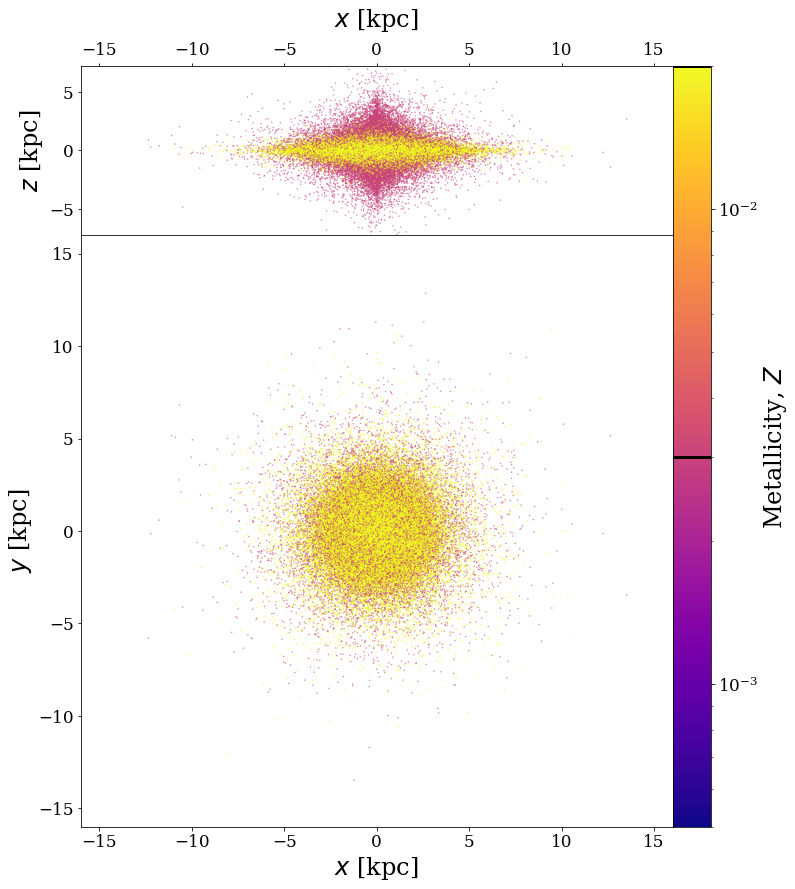
\includegraphics[width=\columnwidth]{../figures/random_simple_galaxy.png}
    \caption{As Fig.~\ref{fig:galaxy_schematic} (right panel), but for the Milky Way model used in \citet{Breivik+2020}.}
    \label{fig:simple_mw}
\end{figure}

When applying this simpler Milky Way model in combination with our fiducial binary physics assumptions (model \modFid{}), we find that the expected number of detections for BHBHs, BHNSs and NSNSs for a 4-year LISA mission is $39$, $39$ and $14$ respectively. Thus the BHBH and BHNS detection rates are only marginally increased from our main findings, but the NSNS detection has increased by nearly a factor of 2.

Moreover, the distribution of parameters within the population, particularly the mass distributions, are notably disparate. By using only two fixed metallicity populations, unphysical artifacts are introduced into distribution of DCO masses (Kummer at al. (in prep)). For example, in Fig.~\ref{fig:bh_mass_simple_mw}, we show the black hole mass distribution produced by the simulation using the simple Milky Way model. Despite the fact that these KDEs use the same bandwidth as Fig.~\ref{fig:fiducial_pdf_distributions}, the distributions show many more sharp transitions, which is a result of pileups occurring at specific masses for specific metallicities. Moreover, the lack of lower metallicities systems means that higher mass systems are not formed and so we see the distributions do not include a high mass tail such as in our fiducial results.

The unphysical artifacts present in the mass distributions can have far-reaching effects since the masses of DCOs affect most other parameters. The inspiral time and SNR are directly dependent on the mass, whilst the uncertainty estimates depend on the SNR. This means that the artifacts can affect the predictions for most distributions of LISA detectable populations.

Overall, we find that previous studies that use Milky Way models analogous to this simpler model may significantly overestimate the LISA NSNS detection rate as well as contain unphysical artifacts in their parameter distributions.

\begin{figure}[htb]
    \centering
    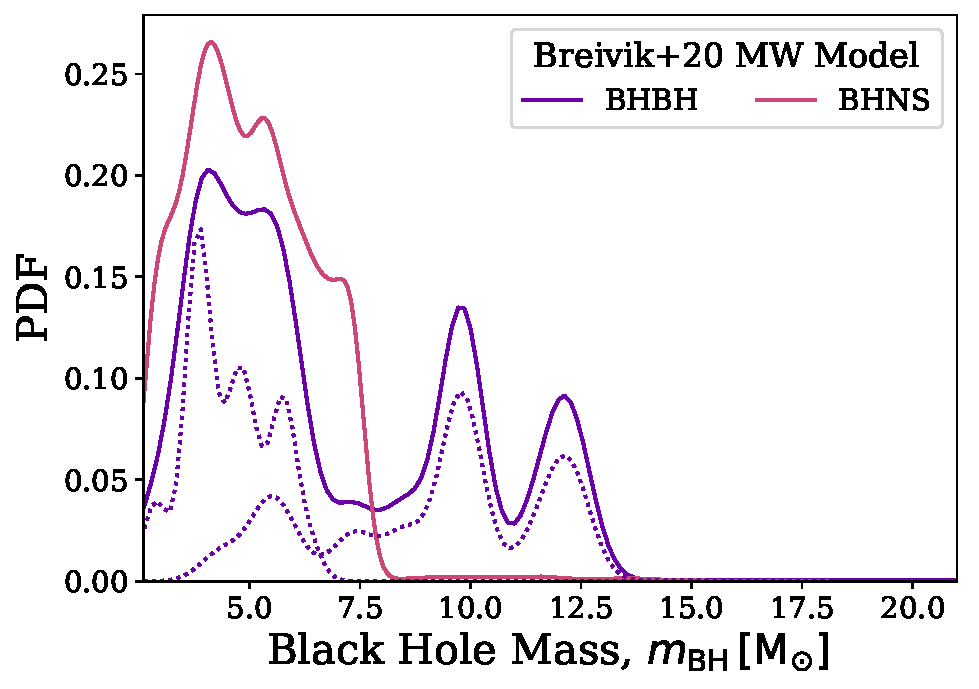
\includegraphics[width=\columnwidth]{../figures/BH_mass_dist_simple_mw.pdf}
    \caption{As Fig.~\ref{fig:fiducial_pdf_distributions} (top left panel), but for the Milky Way model used in \citet{Breivik+2020}.}
    \label{fig:bh_mass_simple_mw}
\end{figure}

\section{Estimating the number of pulsars for a given sky area in SKA}\label{app:ska_area}

In this section, we perform some back-of-the-envelope calculations in order to estimate the number of pulsars that SKA will observe within a given sky area.

First, we consider how many pulsars SKA is likely to detect. \citet{Keane+2015} uses PSRPOPPy \citep{Bates+2014} to simulate the Milky Way pulsar population. They find that for SKA-1, approximately $10000$ pulsars will be discovered. The second phase of SKA, which should be in operation by the time of the LISA mission, would yield a total of $35000$-$41000$ pulsars \citep{Keane+2015}. We use the average, $38000$, in further estimates below. Moreover, we are only interested in pulsars that are part of a binary system. We estimate this pulsar binary fraction as the fraction of known pulsars that are in binaries using the ATNF Pulsar Catalogue\footnote{\url{https://www.atnf.csiro.au/research/pulsar/psrcat}} \citep{Manchester+2005}. $290$ of the $2872$ currently known pulsars are in binary systems and thus we estimate the binary fraction of pulsars as $10\%$. Therefore, we expect that SKA-1 and SKA-2 will detect approximately $1000$ and $3800$ binary pulsars respectively.

Next, we can find the total number of pulsars SKA will detect in a patch on the sky. The total sky area that the SKA mission covers is approximately $5700 \unit{deg^2}$, which is calculated by integrating over the sky for all Galactic longitudes and Galactic latitudes limited to $\abs{b} < 10^\circ$ and $\delta < 45^\circ$, which are the limits on SKA-mid \citep{Keane+2015}. If we assume that the pulsars are found uniformly across the sky, this means that roughly $0.2$ and $0.7$ binary pulsars are expected per square degree for SKA-1 and SKA-2 respectively. Note that the assumption of a uniform distribution is not realistic as pulsars will tend to be far more concentrated in the Galactic centre but we use it to provide an upper bound on these estimates.

Overall, we therefore expect a single pulsar per $5.7 \unit{deg^2}$ and $1.5 \unit{deg^2}$ for SKA-1 and SKA-2 respectively, which correspond to angular resolutions of $\sigma_\theta = 1.3^\circ$ and $\sigma_\theta = 0.7^\circ$.

\clearpage
\onecolumngrid

\section{Supplementary material}

\subsection{Detection rate table}
\begin{table*}[htb]
    \centering
    \caption{The number of detectable binaries in a 4- and 10-year LISA mission for the \nModels{} different model variations and each DCO type. Each value shows the mean and the 1-$\sigma$ Poisson uncertainty.}
    \begin{tabular}{cl|lll|lll}
        \hline
        \multirow{2}{*}{Model} & \multirow{2}{*}{Description} & \multicolumn{3}{c|}{LISA detections (4 year)} & \multicolumn{3}{c}{LISA detections (10 year)} \\ \cline{3-8}
        & & \scriptsize{BHBH} & \scriptsize{BHNS} & \scriptsize{NSNS} & \scriptsize{BHBH} & \scriptsize{BHNS} & \scriptsize{NSNS} \\
        \hline
        A & Fiducial & \confinv{73.7}{8.7}{8.3} & \confinv{42.1}{6.1}{6.9} & \confinv{7.9}{2.9}{3.1}\\
        B & Fixed mass transfer efficiency of $\beta=0.25$ & \confinv{68.6}{8.6}{8.4} & \confinv{22.3}{4.3}{4.7} & \confinv{2.9}{1.9}{2.1}\\
        C & Fixed mass transfer efficiency of $\beta=0.5$ & \confinv{46.8}{6.8}{7.2} & \confinv{8.2}{3.2}{2.8} & \confinv{3.9}{1.9}{2.1}\\
        D & Fixed mass transfer efficiency of $\beta=0.75$ & \confinv{46.8}{6.8}{7.2} & \confinv{7.4}{2.4}{2.6} & \confinv{12.7}{3.7}{3.3}\\
        E & Case BB mass transfer is always unstable & \confinv{69.0}{8.0}{8.0} & \confinv{7.2}{2.2}{2.8} & \confinv{0.2}{0.2}{0.8}\\
        F & Model E + Model K & \confinv{153.8}{12.8}{12.2} & \confinv{147.8}{11.8}{12.2} & \confinv{18.2}{4.2}{3.8}\\
        G & CE efficiency $\alpha = 0.1$ & \confinv{27.8}{4.8}{5.2} & \confinv{2.1}{1.1}{1.9} & \confinv{10.2}{3.2}{2.8}\\
        H & CE efficiency $\alpha = 0.5$ & \confinv{61.7}{7.7}{8.3} & \confinv{28.1}{5.1}{4.9} & \confinv{6.2}{2.2}{2.8}\\
        I & CE efficiency $\alpha = 2.0$ & \confinv{71.6}{8.6}{8.4} & \confinv{38.1}{6.1}{5.9} & \confinv{31.1}{5.1}{5.9}\\
        J & CE efficiency $\alpha = 10.0$ & \confinv{0.0}{0.0}{0.0} & \confinv{0.0}{0.0}{0.0} & \confinv{0.0}{0.0}{0.0}\\
        K & HG donor stars initiating a CE survive CE & \confinv{154.1}{12.1}{12.9} & \confinv{58.9}{7.9}{8.1} & \confinv{9.6}{2.6}{3.4}\\
        L & Fryer rapid SN remnant mass prescription & \confinv{50.2}{7.2}{6.8} & \confinv{70.0}{8.0}{8.0} & \confinv{6.6}{2.6}{2.4}\\
        M & Maximum NS mass = 2.0 ${\rm M_{\odot}}$ & \confinv{95.9}{9.9}{10.1} & \confinv{30.0}{5.0}{5.0} & \confinv{7.1}{3.1}{2.9}\\
        N & Maximum NS mass = 3.0 ${\rm M_{\odot}}$ & \confinv{58.1}{8.1}{7.9} & \confinv{51.7}{6.7}{7.3} & \confinv{8.2}{3.2}{2.8}\\
        O & PISN and pulsational-PISN not implemented & \confinv{75.1}{9.1}{8.9} & \confinv{43.2}{6.2}{6.8} & \confinv{7.9}{2.9}{3.1}\\
        P & $\sigma_{\rm RMS}^{\rm 1D} = 100 \ {\rm km\ s^{-1}}$ for core-collapse supernova & \confinv{82.4}{9.4}{8.6} & \confinv{86.3}{9.3}{9.7} & \confinv{15.4}{4.4}{3.6}\\
        Q & $\sigma_{\rm RMS}^{\rm 1D} = 30 \ {\rm km\ s^{-1}}$ for core-collapse supernova & \confinv{91.5}{9.5}{9.5} & \confinv{142.4}{12.4}{11.6} & \confinv{33.4}{5.4}{5.6}\\
        R & Black holes receive not natal kick & \confinv{85.9}{8.9}{9.1} & \confinv{95.8}{9.8}{10.2} & \confinv{9.7}{2.7}{3.3}\\
        S & Wolf-Rayet wind factor $f_{\rm WR} = 0.1$ & \confinv{75.4}{8.4}{8.6} & \confinv{33.9}{5.9}{6.1} & \confinv{8.8}{2.8}{3.2}\\
        T & Wolf-Rayet wind factor $f_{\rm WR} = 5.0$ & \confinv{0.0}{0.0}{0.0} & \confinv{14.9}{3.9}{4.1} & \confinv{9.6}{3.6}{3.4}\\
        \hline
    \end{tabular}
    \label{tab:detection_rates}
\end{table*}

\subsection{Distribution of eccentric sources on sensitivity curve}
\begin{figure*}[hb]
    \centering
    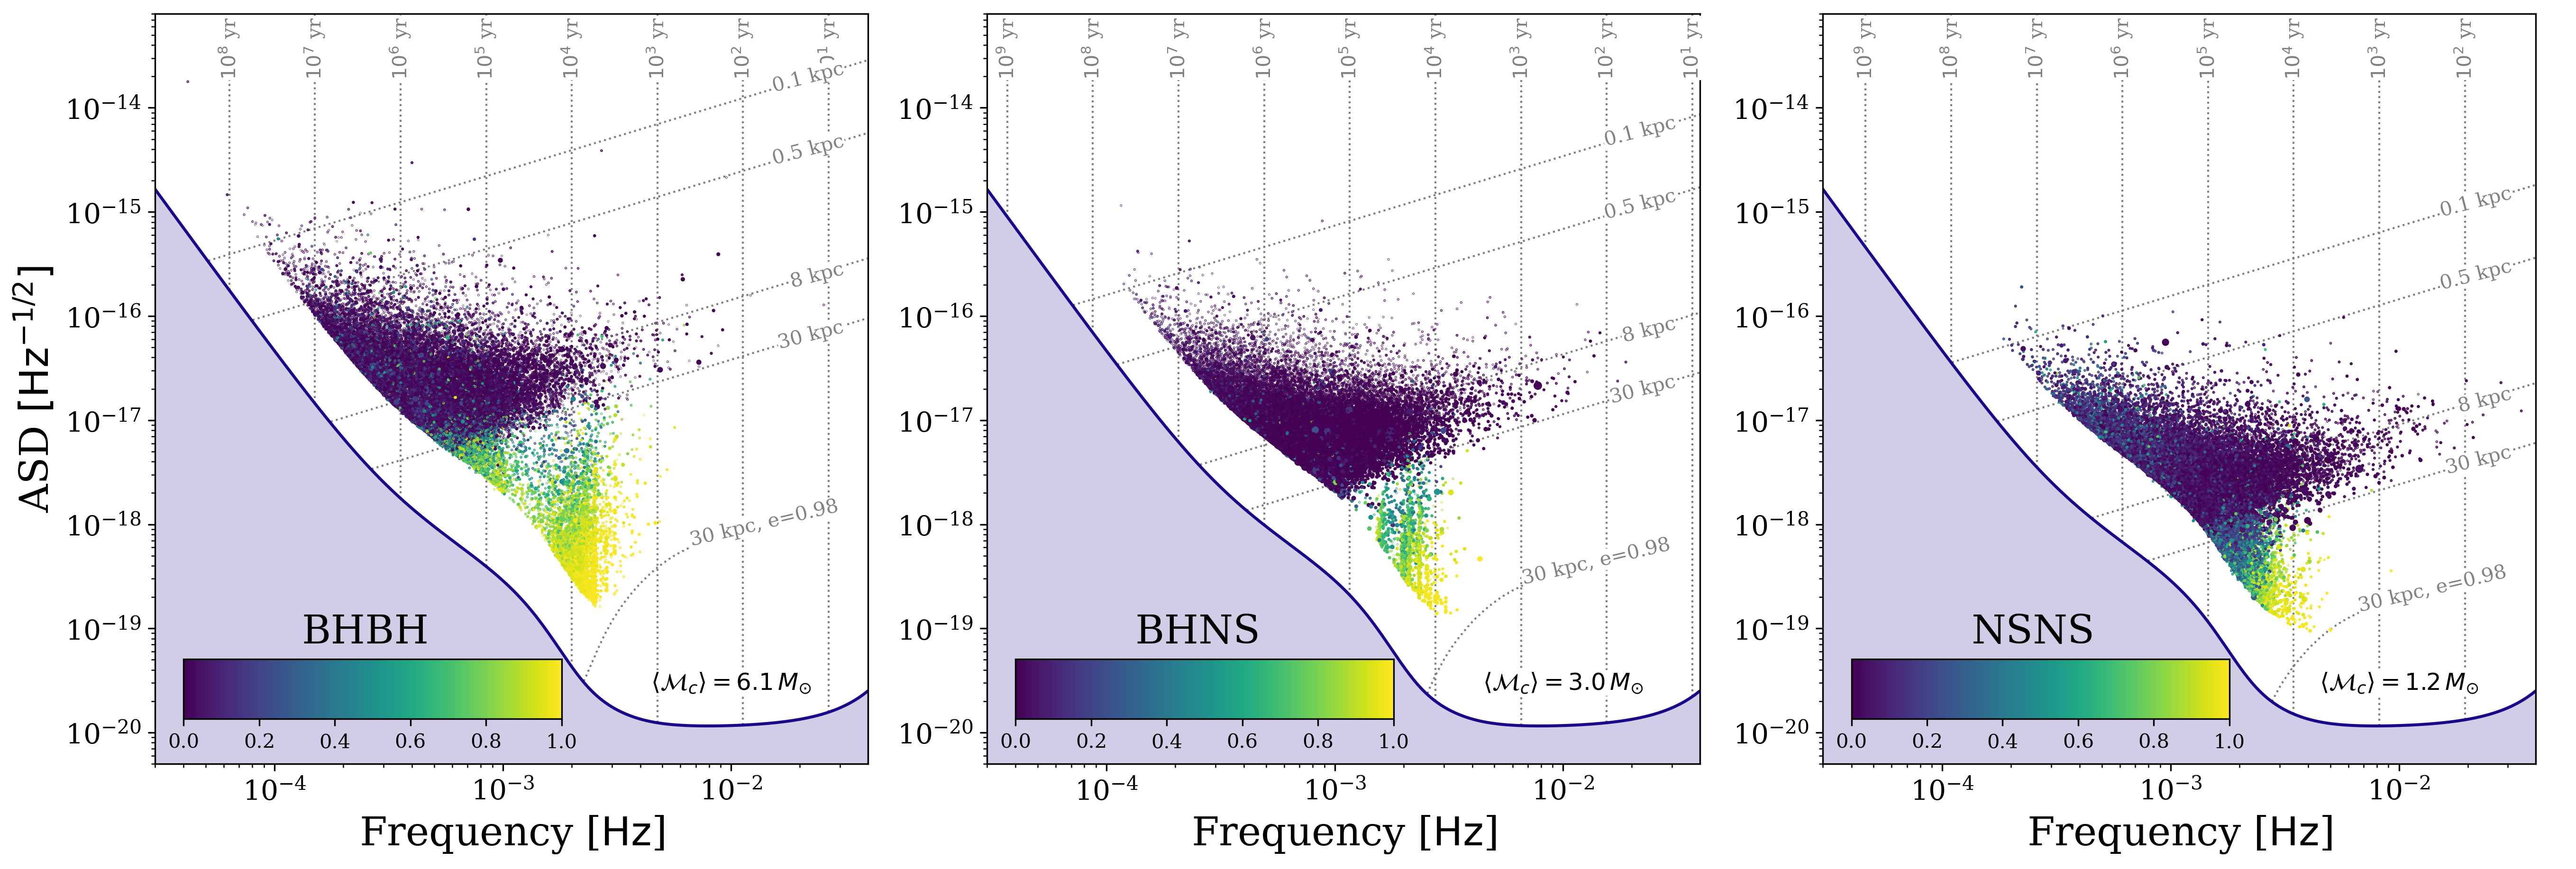
\includegraphics[width=\textwidth]{dcos_on_sc_eccentric_colours.png}
    \caption{As the bottom panels of Fig.~\ref{fig:dcos_on_sc}, but without the density distributions and scatter points are coloured by their eccentricity. We show eccentric sources are located in an offshoot below the $30 \unit{kpc}$ around $2 \unit{mHz}$.}
    \label{fig:dcos_on_sc_ecc_col}
\end{figure*}

\clearpage

\subsection{Formation channels}

\begin{figure}[thb]
    \centering
    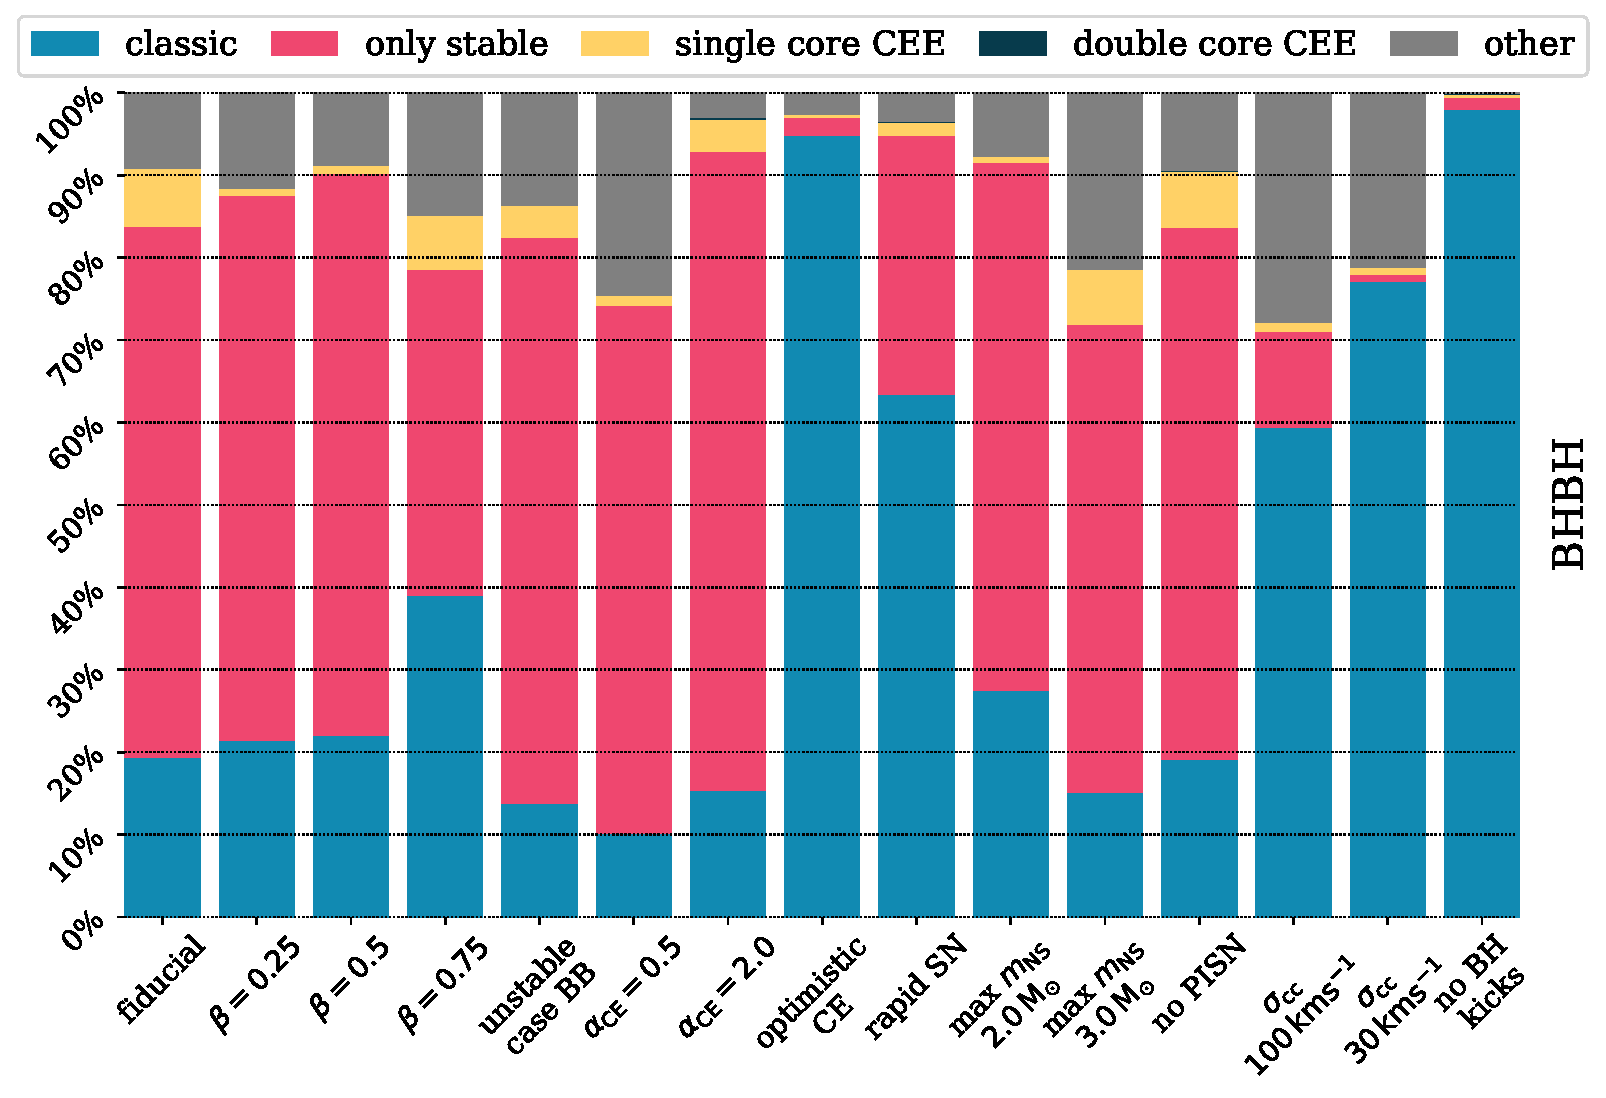
\includegraphics[height=0.28\textheight]{formation_channels_BHBH.pdf}
    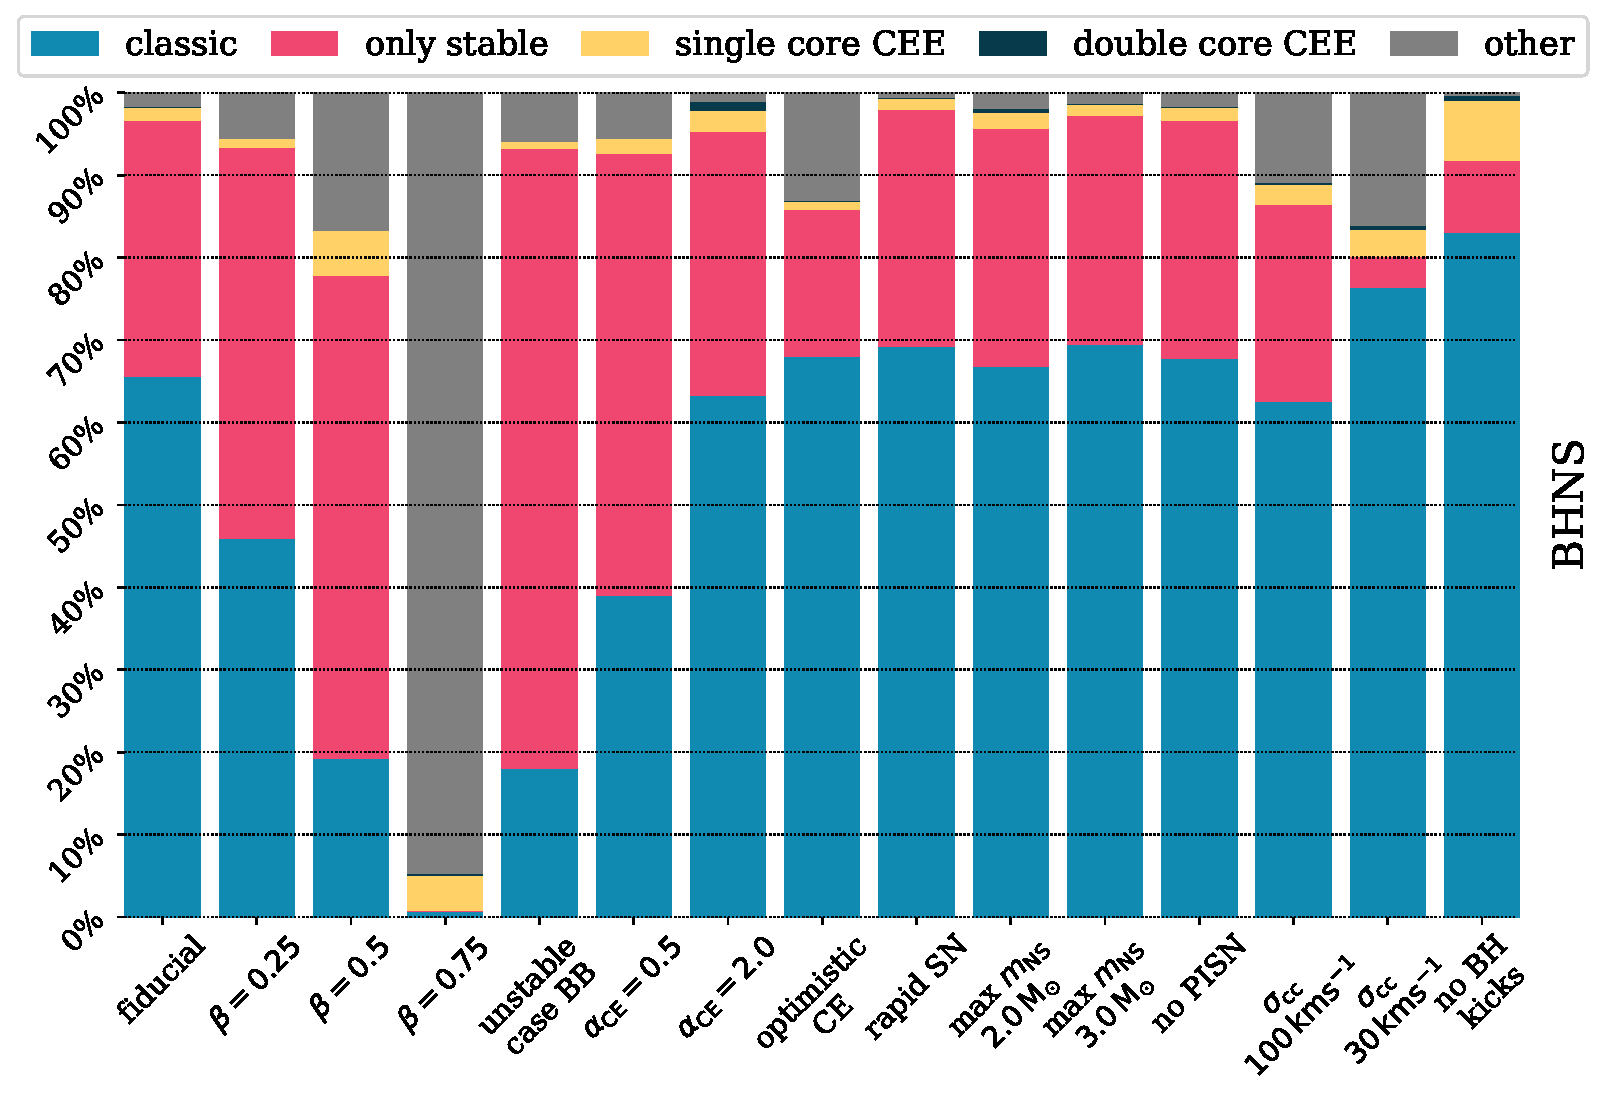
\includegraphics[height=0.28\textheight]{formation_channels_BHNS.pdf}
    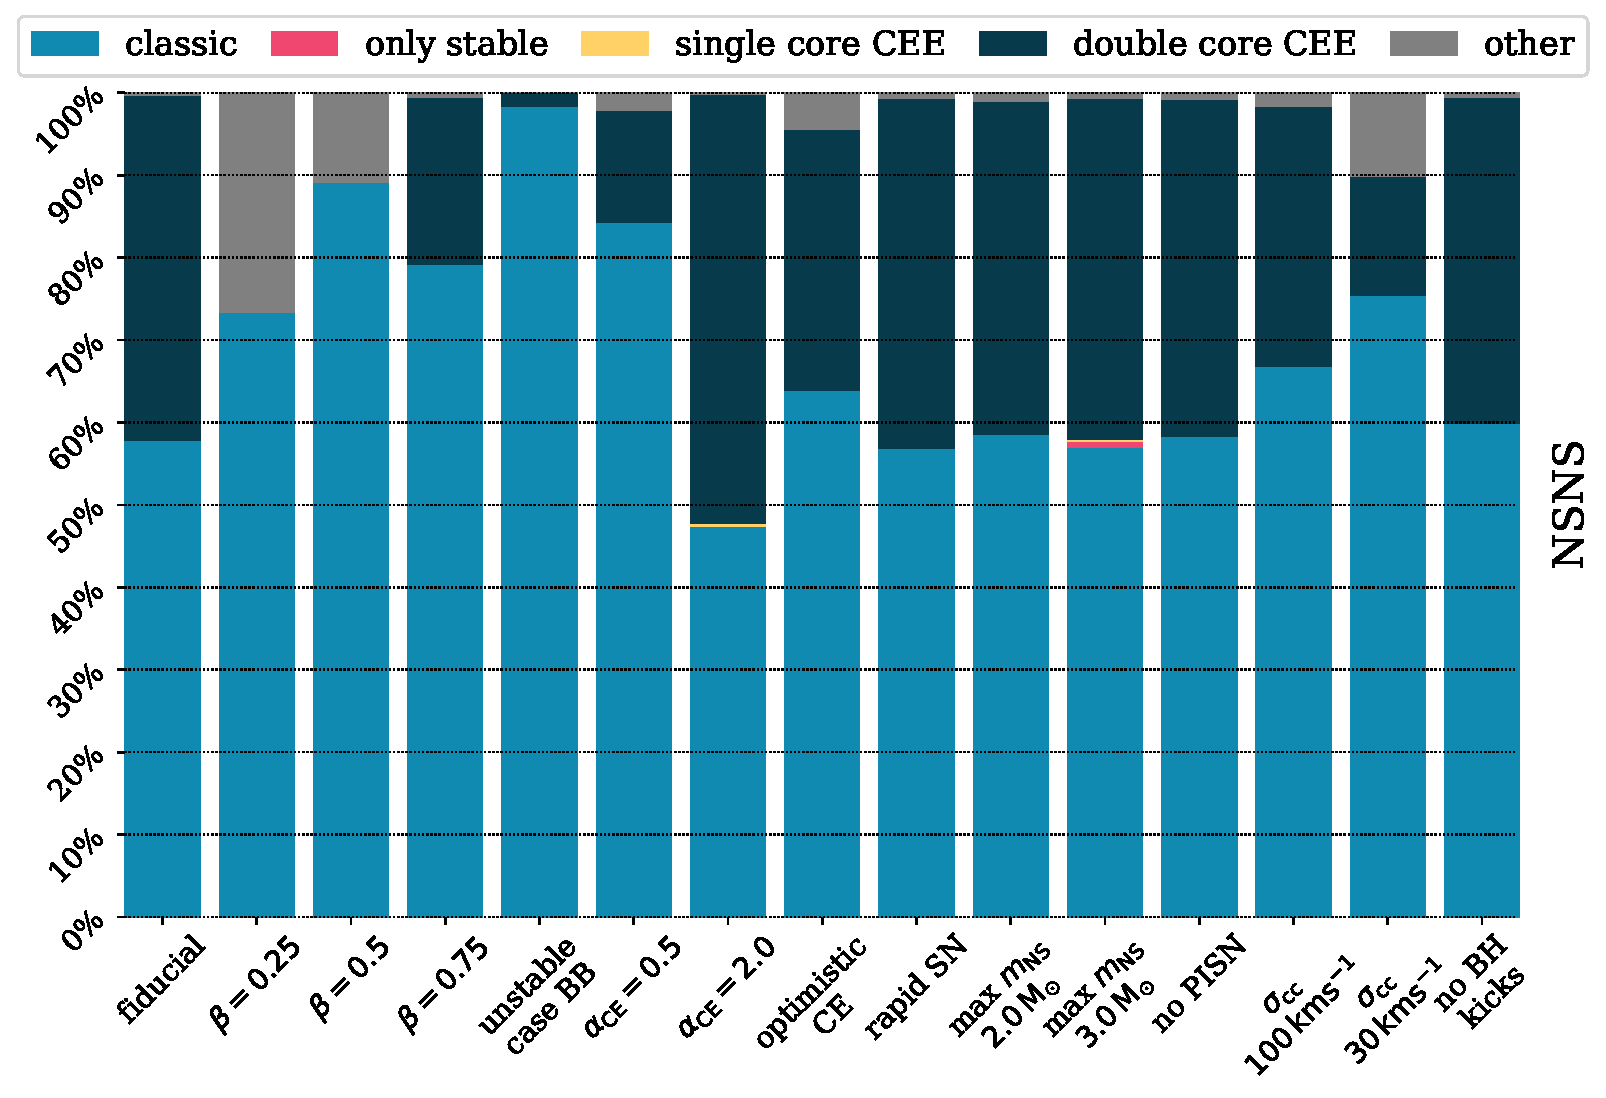
\includegraphics[height=0.28\textheight]{formation_channels_NSNS.pdf}
    \caption{Fraction of each DCO type that is formed through different formation channels for all physics variations. Channels are described in detail in \citet{Broekgaarden+2021}. The classic, single core CEE and double core CEE channels all require at least one common envelope event whilst only `only stable' consists of only stable mass transfer and `other' contains the remaining binaries which are mainly formed from `lucky' supernova kicks that shrink the binary. \todo{Update with new models}}
    \label{fig:formation_channels}
\end{figure}